\chapter{Evaluation}
\label{cha:evaluation}


\section{Validation}

Extensive validation was conducted to ensure the correctness, robustness and reliability of the file server under both normal and adverse conditions. Given the range of supported operations, numerous edge cases and error scenarios arise. Additionally, the presence of multiple clients and asynchronous communication introduces further complexity, requiring testing not only to verify functional correctness but also to ensure that the system maintains consistency and stability under concurrent workloads.

To increase confidence in the correctness of the system as a whole, testing was conducted at multiple levels. Initially, unit testing was used to verify the functionality of individual components in isolation. This enabled a modular development approach, allowing components to be validated incrementally during implementation. Testing at this level also simplified debugging, as errors were easier to localise due to their limited scope and the reduced code surface. 

However, as the system relies heavily on interactions between components and communication between protection domains, integration testing was also necessary. This enabled validation of end-to-end behaviour, ensuring that all operations functioned correctly when executed through the full client–server interface under a range of conditions.

\subsection{Unit Tests}

Unit tests were developed for the core of the file system, including components such as block management, inode management, directory handling and file table operations. These tests focused solely on verifying the correctness of the file server’s data structures and their accesses.

To ensure this isolation, these components were tested by directly invoking their functions outside of the Microkit environment. This allowed inputs and supporting data to be mocked through deterministic flows, and the internal state of the file system to be inspected, enabling correctness to be validated at each stage of execution. Testing regular inputs alongside failure conditions such as resource exhaustion gave confidence that the fundamental building blocks of the file system operated correctly before integration and would not cause wider issues upon failure.
\newpage
For example, one test constructs a mock “indirect block” containing a list of allocated block indices, invokes the indirect-release routine, and then verifies that each referenced block is marked free in the allocation table.


\subsection{Integration Tests}

Once the components were verified, integration testing was used to validate the behaviour of the system as a whole, exercising all file system operations through its regular running microkit environment. Rather than directly inspecting internal state, validation was performed through the responses and error codes returned to clients, such as creating a file then listing the file system. This ensured that testing reflected real system usage and confirmed that correct behaviour was exposed through the public interface.

\subsubsection{Single Client}

These tests exercised the majority of functionality from the client’s perspective, covering the full lifecycle of files, including creation, reading, writing and deletion, without the added complexity of concurrent access. Within this scope, it was possible to verify that invalid client inputs were correctly rejected with appropriate error codes, for example when attempting to delete a non-existent file. Additionally, boundary conditions were tested to ensure correct behaviour under extreme cases, such as reading the maximum supported amount of data.

\subsubsection{Multiple Clients}

To ensure that all clients were serviced correctly and fairly, and that the system operated reliably under load, extended tests were conducted which interleaved operations from multiple clients. This enabled validation of scenarios that cannot be observed in a single-client context, including permission enforcement and modification of shared resources.

As clients execute independently, explicit synchronisation was required. This was achieved through the use of marker files, where clients created files with predefined names that were monitored by other clients. These acted as barriers, allowing coordination of execution order and enabling clients to signal completion of operations to both the server and one another. For example, one test creates a publicly readable file within client 1, after which client 2 attempts to read the file to verify access is permitted. The file is then modified by client 1 to be private, and client 2 subsequently attempts to read it again, verifying that the operation is correctly rejected with a permissions error.

\section{Performance Evaluation}

\subsection{Goals}

The primary goal of this evaluation was to compare the performance characteristics of the synchronous and asynchronous file server designs. In particular, the evaluation aimed to quantify the impact of inter-process communication (IPC) overhead and assess the effectiveness of batching in reducing per-operation cost. Additionally, the behaviour of both systems under multiclient workloads was examined to determine how well each design scales under contention.

\subsection{Metrics}

For the per operation benchmarking, performance was evaluated using the average time per operation, calculated by measuring the total execution time of a long sequence of operations, to amortise any stochastic effects, and dividing by the number of operations performed. For the more realistic workflows, time taken to complete the whole suite was used. These provided consistent bases for comparing synchronous and asynchronous implementations.

Time measurement was performed using the CPU cycle counter, as the low-level execution environment does not provide native timing facilities. The cycle count was recorded before and after each client’s measurable operations, and converted to elapsed time using the processor’s clock frequency. Results were averaged across multiple runs to reduce variance and improve reliability.

In multiclient scenarios, fairness was also considered. This was validated by recording the total time taken by each client to complete its workload, ensuring that no individual client experienced disproportionate delay.

\subsection{Experimental Setup}

All experiments were conducted within the same emulated environment using QEMU on an AArch64 platform, ensuring consistency across all tests. Both synchronous and asynchronous implementations were evaluated under identical conditions, with the same workloads, file sizes and file system state.

For each experiment, the only variables altered were the server design (synchronous or asynchronous), the batching configuration and the number of clients. All operations were validated for correctness during execution to ensure that performance results reflected valid system behaviour rather than erroneous outcomes. During the varied workload, this processing also mimicked non-file I/O that would occur in a typical system, helping to ensure that the measured performance reflects realistic operating conditions.

\subsection{Benchmark Design}

Two benchmark suites were developed to evaluate system performance. The first was designed to isolate and quantify the reduction in communication overhead achieved by the asynchronous server, while the second evaluated overall system performance under more realistic and varied workloads.

This initial aim was achieved through a single-client benchmark that repeatedly executed a single type of operation allowing controlled measurements of individual operation costs for both systems. Both read and write operations were evaluated independently, as they are representative of common file system usage and exhibit differing behaviour. As timing was recorded from the client’s perspective, this included both internal server processing time and communication overhead.

For the asynchronous implementation, the benchmark was executed with varying batch sizes. A batch size of one provided a baseline comparison, ensuring that the asynchronous design does not significantly degrade performance when batching is not possible, which is important as many real workloads contain inherent dependencies. Larger batch sizes allowed evaluation of how batching reduces per-operation cost, identifying the point at which performance improvements become significant and where further increases yield diminishing returns.

As the internal file system operation of both systems are the same, this benchmark also enabled estimation of communication overhead. Let $s$ denote the time taken for a single operation in the synchronous system and $a_n$ the time taken for a batch of $n$ operations in the asynchronous system. Let $x$ represent the internal processing time per operation, and $c_s$ and $c_{a_n}$ the communication overheads. Then:

\begin{equation}
s = c_s + x
\end{equation}

\begin{equation}
a_n = c_{a_n} + n x
\end{equation}

And

\begin{equation}
s \cdot n = c_s \cdot n + n x
\end{equation}

Hence

\begin{equation}
s \cdot n - a_n = c_s \cdot n - c_{a_n}
\end{equation}

Using measured values of $s$ and $a_n$, this relationship allows the difference in communication overhead between the synchronous and asynchronous systems to be quantified across varying batch sizes.

Furthermore:

\begin{equation}
\frac{a_n}{n} = \frac{c_{a_n}}{n} + x
\end{equation}

This formulation also allows analysis of the average cost per operation in the asynchronous system. As the batch size increases, the communication overhead is amortised across multiple operations, causing the per-operation communication cost to decrease. In the limit, the average operation time approaches the internal processing time $x$, indicating that communication overhead becomes negligible. This highlights the fundamental advantage of batching, as it allows the system to approach optimal performance bounded only by computation.

The second benchmark was a multiclient, realistic workload designed to simulate typical file system usage. Multiple clients executed independently, each performing a sequence of  varied operations across many files. This sequence consisted of CREATE, WRITE, CLOSE, OPEN, SEEK, READ and DELETE operations, representing a complete file lifecycle. Operations were interleaved across clients to introduce contention and better reflect real-world usage patterns.

As batching is central to the performance benefits of the asynchronous design, this benchmark was structured to allow batching where it would naturally occur, without artificially constraining the workload. While it is possible to construct workloads with strict dependencies between operations, this would reduce asynchronous behaviour to that of the synchronous system and provide limited insight beyond the single-operation benchmark. Instead, operations were grouped into realistic batches, for example: CREATE | WRITE and CLOSE | OPEN | SEEK and READ and DELETE.

Performance was measured across varying numbers of clients, enabling analysis of scalability, contention and the impact of concurrent access. This approach provided a balanced evaluation, allowing direct comparison of synchronous and asynchronous designs under both controlled and realistic conditions.

\subsection{Results and Analysis}

\subsubsection{Single-Client Per-Operation Benchmark}

\begin{figure}[H]
    \centering
    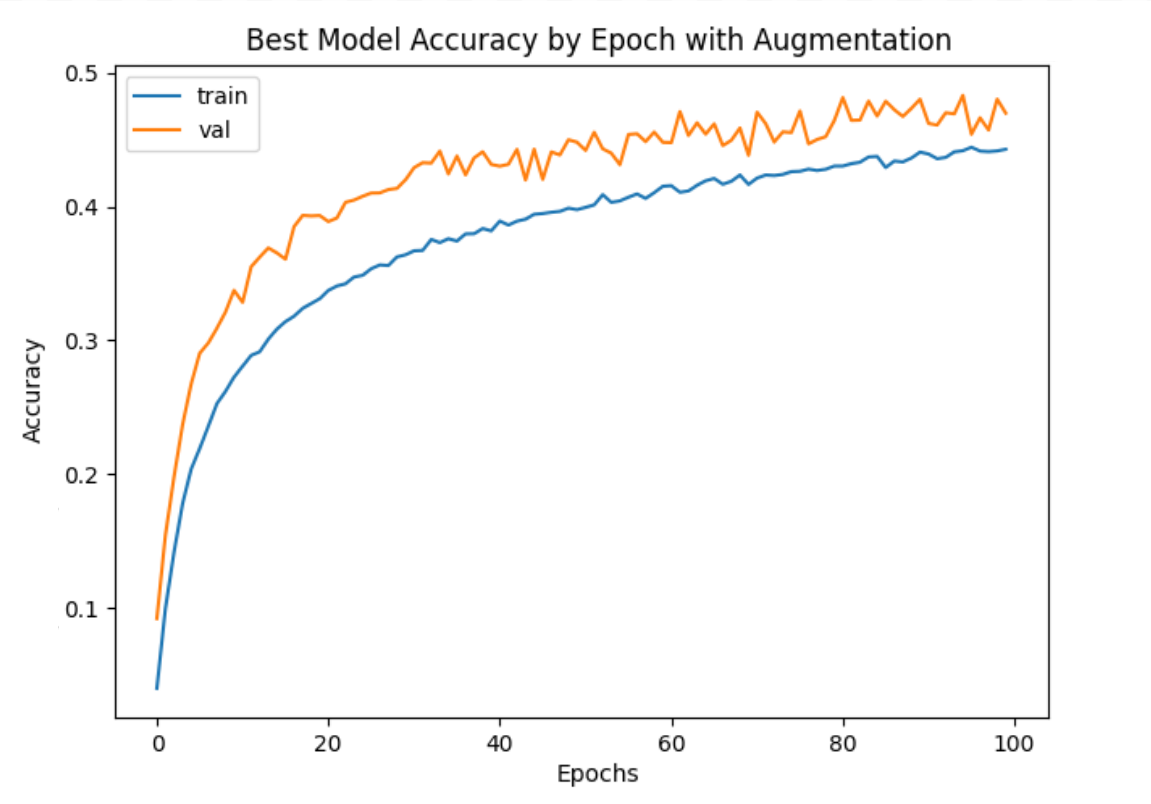
\includegraphics[width=0.7\linewidth]{chapters/images/single_graph.png}
    \caption{Average Time per Operation vs Batch Size (Read and Write)}
    \label{fig:example}
\end{figure}

The synchronous baseline establishes the per-operation cost of IPC without batching. Write operations averaged 186~$\mu$s, while read operations averaged 155~$\mu$s, reflecting the expected asymmetry due to additional data movement and persistence overhead in writes.

When the asynchronous system is configured with a batch size of one, performance is effectively equivalent to the synchronous implementation. Writes measured 187~$\mu$s and reads 158~$\mu$s, indicating that the introduction of asynchronous infrastructure does not impose significant additional overhead in the absence of batching. This validates the design goal that the asynchronous system should degrade gracefully to synchronous-like behaviour when batching is not possible.

As batch size increases, a clear and substantial reduction in per-operation cost is observed. For write operations, the average latency decreases from 187~$\mu$s (batch~=~1) to 74~$\mu$s (batch~=~10), representing approximately a 60\% reduction. Similarly, read operations decrease from 158~$\mu$s to 41--48~$\mu$s, corresponding to a $\sim$70--74\% reduction at optimal batch sizes.

The results exhibit a diminishing returns pattern. The most significant improvements occur between batch sizes 1 and 4:
\begin{itemize}
    \item Write latency drops from 187~$\mu$s to 91~$\mu$s ($\sim$51\% reduction)
    \item Read latency drops from 158~$\mu$s to 63~$\mu$s ($\sim$60\% reduction)
\end{itemize}

Beyond this point, gains become incremental. For example, increasing batch size from 8 to 10 yields negligible improvement for writes (74~$\mu$s $\rightarrow$ 74~$\mu$s) and even slight regression for reads (41~$\mu$s $\rightarrow$ 48~$\mu$s), likely due to increased queuing delay or cache effects.

These results align closely with the analytical model:

\[
\frac{a_n}{n} = \frac{c_{a_n}}{n} + x
\]

As $n$ increases, the amortised communication cost $\frac{c_{a_n}}{n}$ diminishes, and the average operation time approaches the internal processing cost $x$. Empirically, the asymptotic region appears around batch sizes 7--9, suggesting that beyond this range, IPC overhead becomes a minor component of total latency.

Using the relationship:

\[
s \cdot n - a_n = c_s \cdot n - c_{a_n}
\]

we can infer that the synchronous system incurs a linear growth in communication overhead with respect to operation count, whereas the asynchronous system effectively flattens this growth. The widening gap between $s \cdot n$ and $a_n$ as $n$ increases directly quantifies the reduction in IPC overhead achieved through batching.

Notably, read operations benefit more significantly from batching than writes. This suggests that read operations are more heavily dominated by IPC overhead in the synchronous system, whereas writes retain a larger proportion of intrinsic processing cost.

\subsubsection{Multiclient Realistic Workload}

\begin{figure}[H]
    \centering
    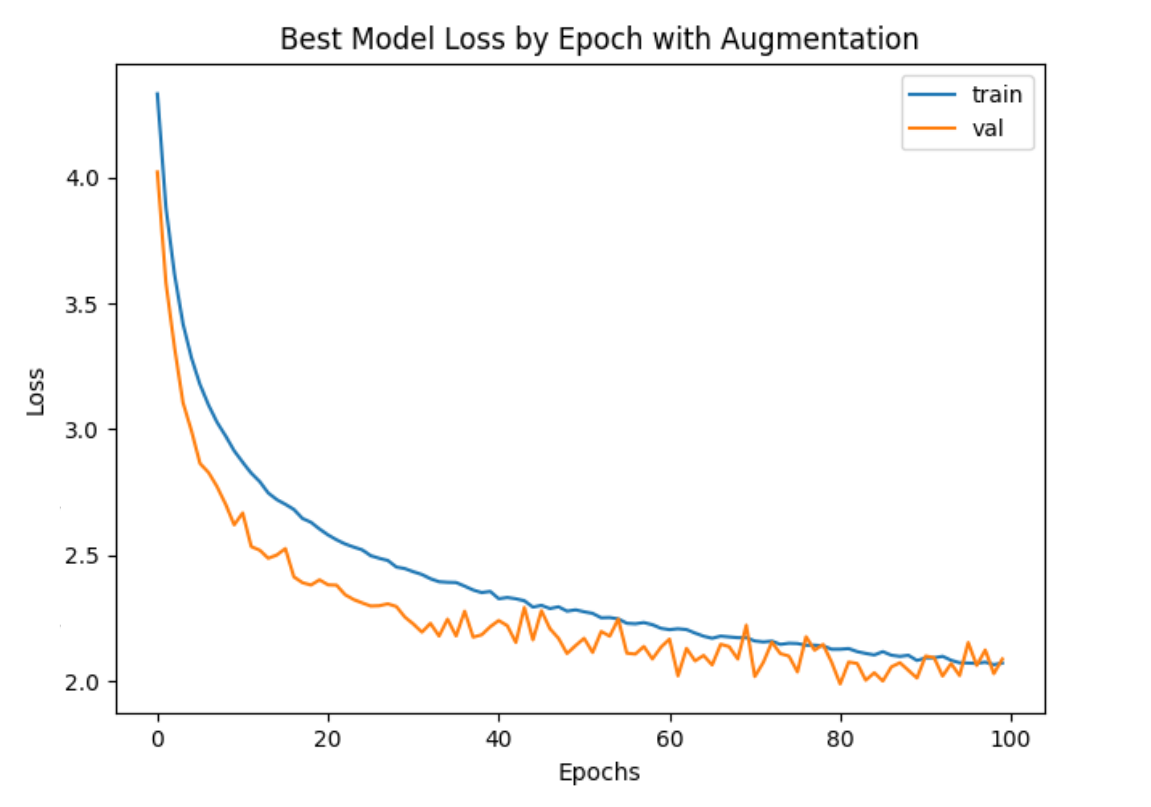
\includegraphics[width=0.7\linewidth]{chapters/images/multi_graph.png}
    \caption{Total Execution Time by Number of Clients (Synchronous vs Asynchronous)}
    \label{fig:example}
\end{figure}

\begin{figure}[H]
    \centering
    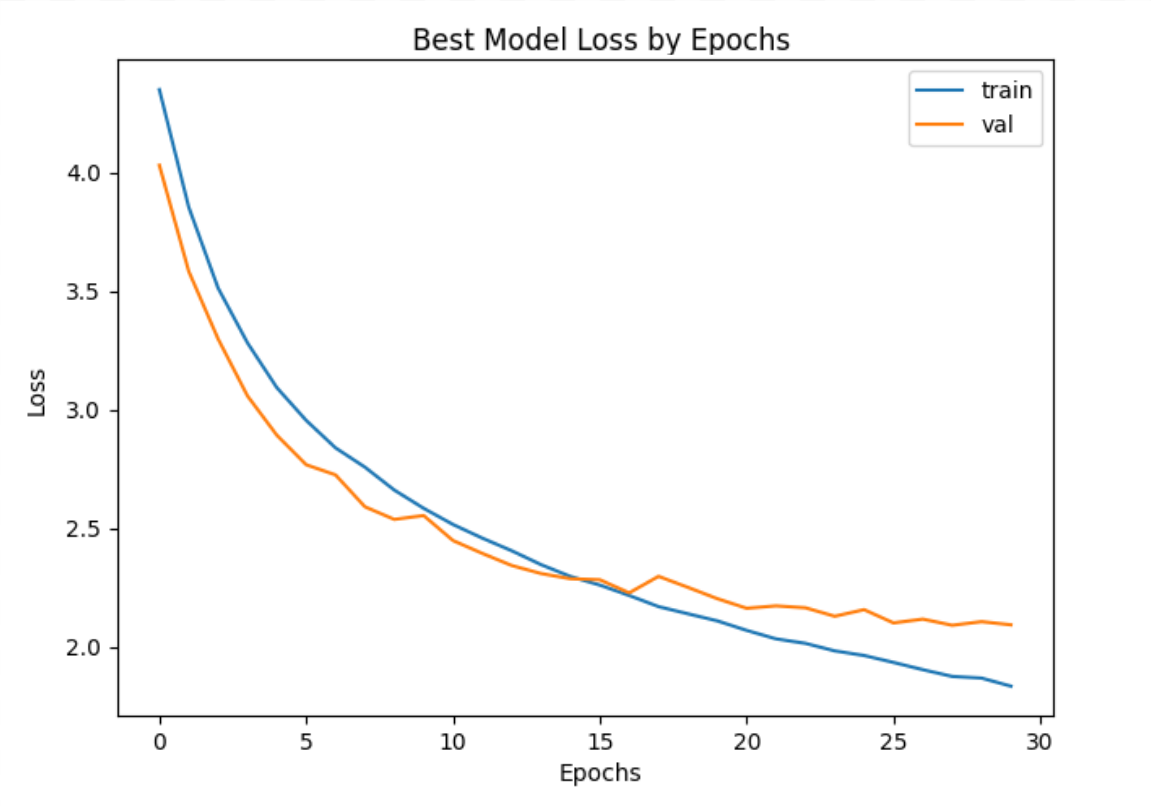
\includegraphics[width=0.7\linewidth]{chapters/images/fairness_graph.png}
    \caption{Execution Times per Client (Fairness Analysis)}
    \label{fig:example}
\end{figure}

Under multiclient workloads, the asynchronous design demonstrates a substantial performance advantage. The synchronous system exhibits total execution times clustered tightly around 25.3--25.7 million~$\mu$s, with per-client averages between 12{,}680--12{,}862~$\mu$s. In contrast, the asynchronous system completes the same workload in approximately 16.0--16.3 million~$\mu$s, with per-client averages between 7{,}844--7{,}941~$\mu$s.

This corresponds to an overall performance improvement of approximately 36--38\%, which is consistent with the reductions observed in the single-operation benchmark when moderate batching is achievable.

Fairness across clients is well maintained in both systems. The variation in per-client average time is minimal:
\begin{itemize}
    \item Synchronous: spread of $\sim$182~$\mu$s ($\sim$1.4\%)
    \item Asynchronous: spread of $\sim$97~$\mu$s ($\sim$1.2\%)
\end{itemize}

This indicates that neither system introduces significant starvation or prioritisation bias. Importantly, the asynchronous design preserves fairness despite its more complex scheduling and batching behaviour.

Another notable observation is the consistency of asynchronous performance across clients. The tighter clustering suggests that batching and concurrent handling smooth out transient delays, reducing sensitivity to contention patterns. In contrast, the synchronous system, while still fair, shows slightly higher variability, likely due to clients serialising on IPC interactions with the server.




